\section{The Discovery of the $W$ and $Z$ Bosons \cite{wz}}
\subsection{Theoretical principles}
In the 1960s Glashow, Salam and Weinberg proposed the electroweak theory $SU(2)_L\times U(1)_Y$. They used the Higgs mechanism to spontanously break the electroweak symmetry into the $U(1)_{em}$. The mass eigenstates after the spontanous symmetry breaking (SSB) are a linear combination of the gauge eigenstates, $B, W^1, W^2$ and $W^3$, and a rotation with the Weinberg angle $\vartheta_W$. They also lead to the mass predictions:
\begin{align*}
	\gamma &= W^3\sin \vartheta_W + B \cos \vartheta_W & m_{\gamma} &= 0\\
	Z^0 &= W^3\sin \vartheta_W - B \cos \vartheta_W & m_Z &= \frac{m_W}{\cos\vartheta_W} = (80\pm25)\si{\GeV}\\
	W^{\pm} &= \frac{1}{\sqrt{2}}(W^1 \pm iW^2) & m_W &= \sqrt{\frac{\pi\alpha}{\sqrt{2}G_F}}\frac{1}{\sin\vartheta_W} = (68\pm40)\si{\GeV}
\end{align*}
The high mass of the weak gauge bosons is the reason that the weak interaction is short ranged. The bosons couple through the conserved weak isospin, which includes all SM particles beside gluons. \\
Till 1975 the weak force was known from radioactive beta and muon decays as well as the discovery of neutral currents. Experimentelle evidence for the weak gauge bosons was still missing. Till the $W^{\pm}$ and the $Z^0$ decay both in hadronic and leptonic final states, the searches were focused on the much cleaner leptonic decays. The only possibility to discover the $W$ boson at lepton colliders was due to pair production which requieres a centor of mass energy of at least $\sqrt{s}\approx \SI{140}{\giga\electronvolt}$. To reach this energies was not realizable with the technology back at the time. This is why the searches were executed at hadron colliders. The boson masses could be reconstructed from the final states with $q\bar{q} \rightarrow W^{+} \rightarrow l^+\nu_l$ and $q\bar{q} \rightarrow Z^{0} \rightarrow l^+l^-$. Since in the 1970s there was a little known about parton distribution functions, the easiest way to make sure that enough antiquarks were present was due $p\bar{p}$ collisions.

\subsection{Experimental Setup}
C.Rubbia, P. McIntyre and D.Cline proposed this possibility to search for massive neutral intermediate vector bosons in 1976. Since CERN already planned LEP, they focused to propose an upgrade of the Super Proton Synchroton (SpS) to a center of mass energy of $\sqrt{s} \approx 400-800 \;\si{\GeV}$ and the use $p\bar{p}$. In 1981 the measurments with the new SppS started.\\
Since the branching fraction of the $Z$ boson into two charged leptons at $\sqrt{s}=\SI{600}{\giga\electronvolt}$ is so small, $3\cdot10^{10}$ antiprotons are needed per day to create one of the requiered events. This rate can be achiebed by firing the Proton Synchroton beam at a target and extracting the antiprotons. The problem is that the antiprotons occupy a too large phase space volume. S. van der Meer invented the process of stochastic cooling to increase the phase space density in 1972. Particles that deviate from their ideal path are registered by an electrode. The signal of this electrode is transmitted to a kicker magnet to bring the particle back to its desired orbit. After this technology was successfully tested, the upgrade of the Sps to the SppS was approved in 1978.\\
The Underground Area 1 experiment (UA1) was the first general-purpuse detector that almost all of the solid angle. The problem is that they used a dipol magnet which lead to false discoveries like monojets. The second experiment (UA2) had to be cheaper and therefore missed a central magnet and muon chambers. They concentrated on the calorimeter to optimize it for the detection of electrons. Both experiments were used to verify the results of each other.

\subsection{Measurements}
Both experiments searched for the decay $W^{\pm} \rightarrow \ e^{\pm} + \overset{\textbf{\fontsize{4pt}{4pt}\selectfont(---)}}{\nu}_e$. They had to reconstruct the missing transverse momenta $\vec{p}_{\text{T}}^{\text{miss}}$ to take advantage of the involved neutrino. The following applies to the transverse pulses $\sum_{\text{cells}}\vec{p}_{\text{T}}=0$ in the case of a perfect measurement. Therefore the missing transverse momentum is equivaltent to $\vec{p}_{\text{T}}^{\text{miss}} = \sum_{\text{cells}}\vec{p}_{\text{T}}$.\\
The data for the $W$ boson search were taken at a 30-day run and delivered approximate 2000 triggered events. Both collaborations searched for one isolated charged track that deploys $E_{\text{T}}>\SI{15}{\GeV}$ in an electromagnetic cluster. UA1 required an energy deposit below \SI{600}{\GeV} in the hadronic calorimeter and UA2 checked if the shower topology matches the expactation for an isolated electron along the track. This led to 39 UA1 events and 4 UA2 events. Events with high transverse momentum electrons seemed to be correlated to high missing transverse momenta events.  Further cuts were applied to access the significance if correlation. The UA1 requiered a $\vec{p}_{\text{T}}^{\text{miss}} >\SI{15}{\GeV}$ together with $E_{\text{T}}>\SI{15}{\GeV}$ and UA2 $\vec{p}_{\text{T}}^{\text{miss}}/E_{\text{T}} \approx 1$. They also manually removed events were jets or limited detector coverage contributed to the missing tranverse momentum. This led 6 UA1 and 4 UA2 events.
The UA1 collaboration considered three sources of background. The one produced due hadrons was eliminated by rejecting tracks with hadronic signature. The number of electron pair production and missing one was nearly zero. And the last was due to heavy flavour production that decay semi leptonic. The signature would just be the same if all other particles would have been missed, which is extremly unlikely. This led to the conclution that no background process could produce the 6 reminding events. In both cases the events were considered as the discovery of the $w$ boson with a mass off
\begin{align*}
	m_W &= 81\pm 5\,\si{\GeV} \;\;(\text{UA1}) & m_W &= 80^{+10}_{-6} \,\si{\GeV} \;\;(\text{UA1})
\end{align*}
Both collaboration also fitted a theory prediction assuming a V-A coupling for the $W$ boson to the tranverse $W$ momentum (UA1) or $E_{\text{T}}(\vartheta)$ (UA2) distribution which in both cases fitted the data.

\begin{wrapfigure}{l}{0.35\textwidth}
    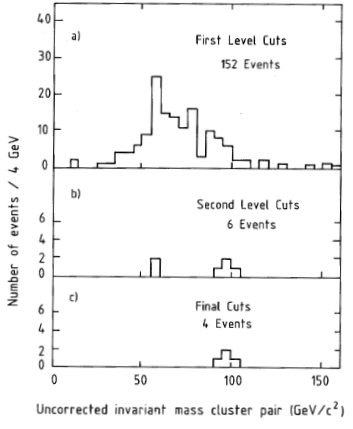
\includegraphics[width=0.33\textwidth]{graphics/Z.png}
    \caption{Invaraint mass distribution of the lepton pairs after subsequent cuts in the UA1 analysis.\cite{wz}}
		\label{fig:Z}
  \end{wrapfigure}
  \FloatBarrier
Again both collaborations searched for the same decay $Z^0 \rightarrow l^+l^-$. The search of the UA2 collaboration was detector specific and led to 4 consistent $e^+e^-$ events. The UA1 experiment had a different analysis strategy. First they requiered two electromagnetic cluster, where each has \SI{25}{\GeV} or more. This led to 152 $e^+e^-$ evnts. Requiering isolated tracks with a tranverse momentum of $p_{\text{T}}>\SI{7}{\GeV}$ led just 6 remaining events. The third and last step was that less than \SI{800}{\MeV} show up in the hadronic calorimeter to suppress the hadronic background. In the end the UA1 collaboration found 4 $e^+e^-$ events and 1 $\mu^+\mu^-$ event. These led to the discovery of the $Z$ boson with an mass of
\begin{align*}
	m_Z &= 92.5 \pm 2.5(\text{stat.})\pm 3.0(\text{syst.})\;\si{\GeV} \;\; (\text{UA1})\\
	m_Z &= 91.9 \pm 1.3(\text{stat.})\pm 1.4(\text{syst.})\;\si{\GeV} \;\; (\text{UA2})
\end{align*}
In 1984 C.Rubbia and S. van der Meer were awarded with the Nobel prize for their work leading to the discovery of the $W$ and the $Z$ boson.
Shortly after this discovery CERN began to opperate the LEP collider. Since lepton colliders provide cleaner events with far less jets, it was possible to perform high precision measurements that were all consistent with the SM. The measurement of the $W$ mass at the LHC is far more challening for example due to the large number of interaction per beam crossing. Never the less the uncertainties have been further reduced. The weak sector is still an interesting topic since e.g. FCNC are one of the few measurments that show tensions to the SM predictions.
